\chapter{Preliminares}

La ciencia de datos es el campo de la aplicacion de tecnicas analiticas avanzadas y principios cientificos para extraer información valiosa de los datos,  teniendo como objetivo principal la extración, análisis y comunicación de información útil a partir de los datos. Esta combina la estadística, la informatica y el pensamiento crítico para extraer información valiosa y significativa de los datos. Para un analisis de datos son necesarios conocimientos en matemáticas, estadística, programación, inteligencia artificial, aprendizaje automático y conocimiento en diversas areas de aplicacion, para esta caso es nesesario incursionar en conocimientos de genomica y metagenomica.\\

En la microbiología un factor de estudio son las interacciones entre microorganismos en un ambiente natural, ya que en su mayoría estos estudios se realizan en laboratorios. Por lo tanto, los avances tecnológicos nos llevan a métodos de secuenciación de ADN. Una de las plataformas más usadas y conocidas en el campo de la metagenómica es Illumina. Con este tipo de herramientas es posible analizar el ADN extraído directamente de una muestra en vez de microorganismos cultivados individualmente. \\

Phylogenetica, es el estudio de la vida evolutiva y las relaciones entre organismos y grupos de organismos. Este análisis se centra en temas de estudio como la diversidad, evolución, ecología, y genomas; y nos ayuda a comprender como genes, genomas y especies evolucionan. Parte importante de este estudio, es la identificación, clasificación y denominación de organismos biológicos; y a este campo se le llama Taxonomía,  principalmente Calr Linnaeus (El padre de la taxonomía) creo 7 niveles taxonómicos (Reino, Phylum, Clase, Orden, Familia, Género y Especie) a los cuales le agregaron el dominio, como el octavo grupo taxonómico más grande, dividido en Arqueas, Bacterias y Eukarya. \\

La metagenómica...\\

En metagenómica existen dos enfoques para la secuenciación de microorganismos, “Amplicón 16S rRNA” y “Shotgun”.  La secuenciación por amplicon  16S fue el primer método de secuenciación metagenómica altamente aceptado, tiene muchas ventajas: el gen 16S está presente en todas las bacterias y arqueas, contiene las regiones necesarias para un buen análisis de PCR altamente conservadas,  existen conjuntos de primers altamente estudiados para amplificar la mayoría de los organismos, ya se encuentran disponibles bases de datos públicas y bien seleccionadas que permiten una buena comparación, la secuenciación por 16S es relativamente barata y simple; aunque posee algunas desventajas: el gen 16S este no está presente en los genes de hongos, por lo que no es bueno este método cuando se desea trabajar con hongos, existe una probabilidad de aumentar un error de sesgo al no elegir el conjunto de primers adecuado para el organismo a analizar. \\

Para realizar una secuenciación por 16S, antes se deben seguir una serie de pasos para la preparación de la muestra biológica y la extracción del ADN: colecta de la muestra, extracción del ADN, preparación de la librería. Para la colecta de las muestras se deben tener en cuenta las necesidades del experimento y los resultados esperados, estimar el número de muestras necesarias y considerar el método de almacenamiento; todo esto para garantizar la calidad de los datos. Existen varios métodos y herramientas para realizar la extracción del ADN. Se necesita una preparación de bibliotecas de datos genómicos para la comparación de las secuencias. Luego de esto, se continúa con la secuenciación de las muestras, para lo cual existen varias herramientas y una de las más usada es Ilumina que ofrece unamayor cobertura a menor costo. Y por último se realiza un control de calidad, del cual los principales objetivos son mejorar la precisión del análisis y prevenir la sobreestimación de los datos, el control de calidad puede incluir: la detección y eliminación de quimeras artificiales, filtrado de secuencias de baja calidad y reads muy cortos y eliminación de ruido. \\

Luego de obtener las secuencias , se requiere identificar el grupo taxonómico para cada secuencia. Para esto se conocen dos enfoques principales: uno basado en filotipos, que como su nombre lo indica, se agrupa directamente en función de la similitud con los filotipos. Y por otro lado, uno basado en OTU’s (Unidades Taxonómicas Operacionales) los cuales agrupan secuencias según la similitud entre OTU’s. El método de agrupación por OTU’s supera al basado en filotipos, pero también tiene ciertas limitaciones, ya que es relativamente costoso computacionalmente y requiere mucha memoria. Un OTU se define entre el mismo cluster por un porcentaje de similitud, siendo 97\% un porcentaje común a nivel de especie. Estos OTU son obtenidos mediante clusterización, para lo cual ya existen varios métodos y algoritmos posibles. (Xia et al., 2018) \\

Los niveles taxonómicos...\\

\begin{figure}[h]
\centering
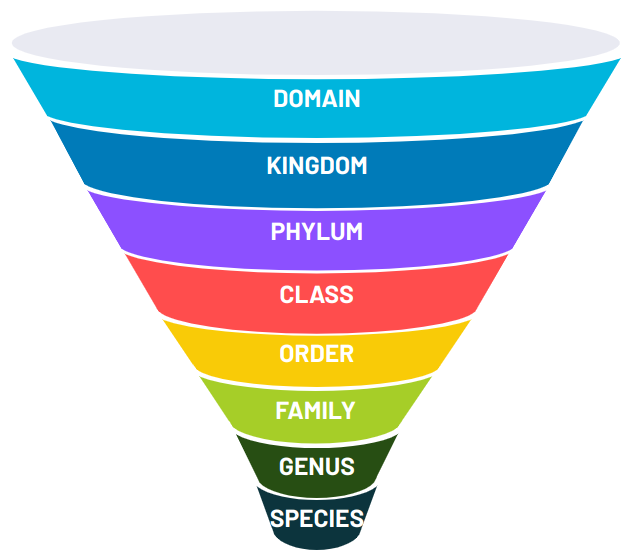
\includegraphics[scale=0.3]{Img/cap1/taxonomic.png}
\caption{Niveles taxonómicos}
\end{figure}

El microbioma se refiere a la comunidad de microorganismos, incluyendo bacterias, virus, hongos y organismos unicelulares, que habitan en un entorno o en un organismo en particular.\\

Kraken, es una herramienta de clasificación de secuencias de ADN metagenómico, mediante alineación exacta de k-meros, asignándoles etiquetas taxonómicas, con gran exactitud y velocidad (\cite{wood2014kraken}).  Este crea su base de datos de consulta, en base a una biblioteca de datos metagenómicos e información taxonómica de NCBI. \\

Kraken deja sin clasificar las secuencias que no tienen k-meros en la base de datos precalculada. \\

Kraken nos entrega una línea por cada read, que contiene 5 ítems separados por tabulaciones. En donde en primer lugar tenemos si el read quedó clasificado o no clasificado (C/U), luego tendremos el nombre del read (este es el ID de la secuencia, el encabezado del archivo FASTA o FASTQ de entrada), la etiqueta taxonómica asignada por kraken (0 en caso de que la secuencia no quede clasificada), longitud de la secuencia en pares de bases (bp), y por último una lista delimitada por espacios que indica el mapeo LCA de cada k-mero de la secuencia (Id taxonómico : \# de k-meros) \\

Para saber todo su ID taxonómico kraken tiene la herramienta (kraken\_translate), el cual luego de los resultados de kraken y con la misma base de datos nos genera una lista de los reads, y el id taxonómico en nombre completo. Y una herramienta complementaria (--mpa-) aparte de esta,nos muestra la salida ordenada por categoría taxonómica (root\_Super Kingdom, d\_kingdom, p\_phylum, c\_class, o\_order, f\_family, g\_genus, s\_species). (Wood \& Salzberg, 2014)  \\

BRACKEN : Bayesian Reestimation of Abundance after Classification with kraKEN: Calcula la abundancia de especies, géneros u otras categorías taxonómicas a partir de las secuencias de ADN recopiladas en un experimento de metagenómica .(\cite{lu2017bracken})  \\

Hace estimaciones probabilísticas en las salidas de kraken para completar las asignaciones al nivel taxonómico que se requiera ,y así lograr una estimación de abundancias más eficaz. Puede producir estimaciones precisas de abundancia a nivel de especie y género incluso cuando una muestra contiene múltiples especies casi idénticas.   \\


Kaiju es un programa para clasificacion taxonomica de lecturas de secuenciación de alto rendimiento,  a partir de la secuenciacion del genoma completo fde ADN metagenomico.  \\

CAMISIM es un simulador de secuencias metagenómicas, este software puede simular una amplia variedad de comunidades microbianas y conjuntos de datos metagenomicos, este algoritmo se divide en tres partes, la primera es el diseño de la comunidad, aqui se crean dichos datos a partir de perfiles taxonomicos de novo o de una base de datos genomicos dada (\cite{fritz2019camisim}). Para el diseño a partir de perfiles taxonomicos, se incluye una base de datos de la taxonomia de NCBI (National Center for Biotechnology Information), y se proporcionan en formato BIOM (Biological Observation Matrix format); estos perfiles pueden incluir taxones de bacterias,arqueas y eucariotas asi como virus. Para el diseño de comunidad de novo, se necesitan genomas en formato .fasta y un archivo de mapeo que contenga ID taxonomico (de NCBI) y OTU para cada genoma.  \\

En segunda parte se basa en la simulacion del metagenoma, los conjuntos de datos del metagenoma se generan a partir de los perfiles de abundancia y genomas del paso anterior; las longitudes de los reads y los tamaños de los insertos se pueden variar para algunos simuladores. Para cada conjunto de datos, CAMISIM genera archivos FASTQ y un archivo BAM.  \\

Y por ultimo en la tercera parte se tiene la creación y posprocesamiento de estandares de oro de ensamblaje y agrupacion, a partir de los datos del metagenoma simulado,los archivos FASTQ y BAM. CAMISIM genera los estándares de oro del genoma y el taxón para las lecturas y los contigs ensamblados, respectivamente. Estos especifican el genoma y el linaje taxonómico al que pertenecen las secuencias individuales. Todas las secuencias se pueden anonimizar y mezclar (pero rastrear durante todo el proceso), para permitir su uso en desafíos de evaluación comparativa.  \\

\begin{itemize}
    \item CAMISIM es un programa flexible para simular una gran variedad de comunidades microbianas y muestras de metagenomas. 
    \item Posee un conjunto de funciones completo para simular comunidades microbianas realistas y conjuntos de datos de metagenomas.
    \item Exploraron el efecto de las propiedades específicas de los datos en el rendimiento del ensamblador.
\end{itemize}

TIPOS DE FORMATOS DE LOS ARCHIVOS
JSON
BIOM
FASTA
FASTQ
...
QUE ES?
QUE DATOS CONTIENEN?
QUE ES UN SAM_DATA
